% 2024 天津 第18题(2) 解答示意图：椭圆 x^2/12+y^2/9=1 与一条过 C(0,-3/2) 的代表弦 PQ
\usetikzlibrary{arrows.meta}
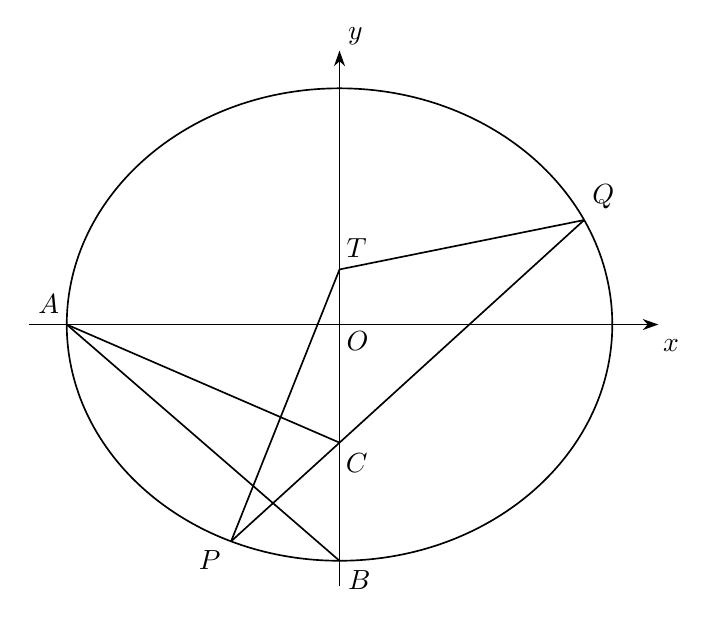
\begin{tikzpicture}[x=1cm,y=1cm,line width=.6pt,font=\normalsize,
  axis/.style={line width=.6pt,-{Stealth[length=2.0mm,width=1.4mm]}},
  curve/.style={line width=.6pt},
  seg/.style={line width=.6pt},
  label/.style={inner sep=0pt,font=\normalsize}]
\coordinate (O) at (0,0);
\coordinate (A) at (-3.4641016151,0);
\coordinate (B) at (0,-3);
\coordinate (C) at (0,-1.5);
\coordinate (T) at (0,0.6996470784);
\coordinate (P) at (-1.3767892557,-2.7528782227);
\coordinate (Q) at (3.1067176506,1.3271130621);
\coordinate (xmin) at (-3.95,0);
\coordinate (xmax) at (4.05,0);
\coordinate (ymin) at (0,-3.32);
\coordinate (ymax) at (0,3.48);
\draw[curve] (O) ellipse [x radius=3.4641016151, y radius=3];
\draw[axis] (xmin)--(xmax);
\draw[axis] (ymin)--(ymax);
\draw[seg] (A)--(B);
\draw[seg] (A)--(C);
\draw[seg] (T)--(P);
\draw[seg] (T)--(Q);
\draw[seg] (P)--(Q);
\node[label,anchor=south east] at (-3.55,0.13) {$A$};
\node[label,anchor=north west] at (0.10,-3.12) {$B$};
\node[label,anchor=north west] at (0.07,-1.63) {$C$};
\node[label,anchor=north west] at (0.08,-0.08) {$O$};
\node[label,anchor=south west] at (0.08,0.84) {$T$};
\node[label,anchor=north east] at (-1.50,-2.86) {$P$};
\node[label,anchor=south west] at (3.20,1.46) {$Q$};
\node[label,anchor=north west] at (4.10,-0.18) {$x$};
\node[label,anchor=south west] at (0.10,3.54) {$y$};
\end{tikzpicture}
